%
% Main document
% ===========================================================================
% This is part of the document "Project documentation template".
% Authors: brd3, kaa1
%

%---------------------------------------------------------------------------
\documentclass[
	a4paper,					% paper format
	10pt,							% fontsize
	twoside,					% double-sided
	openright,				% begin new chapter on right side
	notitlepage,			% use no standard title page
	parskip=half,			% set paragraph skip to half of a line
]{scrreprt}					% KOMA-script report
%---------------------------------------------------------------------------

\raggedbottom
\KOMAoptions{cleardoublepage=plain}			% Add header and footer on blank pages


% Load Standard Packages:
%---------------------------------------------------------------------------
\usepackage[standard-baselineskips]{cmbright}

\usepackage[ngerman]{babel}										% german hyphenation
%\usepackage[latin1]{inputenc}  							% Unix/Linux - load extended character set (ISO 8859-1)
\usepackage[ansinew]{inputenc}  							% Windows - load extended character set (ISO 8859-1)
\usepackage[T1]{fontenc}											% hyphenation of words with �,� and �
\usepackage{textcomp}													% additional symbols
\usepackage{ae}																% better resolution of Type1-Fonts 
\usepackage{fancyhdr}													% simple manipulation of header and footer 
\usepackage{etoolbox}													% color manipulation of header and footer
\usepackage{graphicx}                      		% integration of images
\usepackage{float}														% floating objects
\usepackage{caption}													% for captions of figures and tables
\usepackage{booktabs}													% package for nicer tables
\usepackage{tocvsec2}													% provides means of controlling the sectional numbering
\usepackage{rotating}
\usepackage{multirow}
%---------------------------------------------------------------------------

% Load Math Packages
%---------------------------------------------------------------------------
\usepackage{amsmath}                    	   	% various features to facilitate writing math formulas
\usepackage{amsthm}                       	 	% enhanced version of latex's newtheorem
\usepackage{amsfonts}                      		% set of miscellaneous TeX fonts that augment the standard CM
\usepackage{amssymb}													% mathematical special characters
\usepackage{exscale}													% mathematical size corresponds to textsize
%---------------------------------------------------------------------------

% Package to facilitate placement of boxes at absolute positions
%---------------------------------------------------------------------------
\usepackage[absolute]{textpos}
\setlength{\TPHorizModule}{1mm}
\setlength{\TPVertModule}{1mm}
%---------------------------------------------------------------------------					
			
% Definition of Colors
%---------------------------------------------------------------------------
\RequirePackage{color}                          % Color (not xcolor!)
\definecolor{linkblue}{rgb}{0,0,0.8}            % Standard
\definecolor{darkblue}{rgb}{0,0.08,0.45}        % Dark blue
\definecolor{bfhgrey}{rgb}{0.41,0.49,0.57}      % BFH grey
%\definecolor{linkcolor}{rgb}{0,0,0.8}     			% Blue for the web- and cd-version!
\definecolor{linkcolor}{rgb}{0,0,0}        			% Black for the print-version!
%---------------------------------------------------------------------------

% Hyperref Package (Create links in a pdf)
%---------------------------------------------------------------------------
\usepackage[
	pdftex,ngerman,bookmarks,plainpages=false,pdfpagelabels,
	backref = {false},										% No index backreference
	colorlinks = {true},                  % Color links in a PDF
	hypertexnames = {true},               % no failures "same page(i)"
	bookmarksopen = {true},               % opens the bar on the left side
	bookmarksopenlevel = {0},             % depth of opened bookmarks
	pdftitle = {Smoilet},	   	% PDF-property
	pdfauthor = {us},        					  % PDF-property
	pdfsubject = {LaTeX Template},        % PDF-property
	linkcolor = {linkcolor},              % Color of Links
	citecolor = {linkcolor},              % Color of Cite-Links
	urlcolor = {linkcolor},               % Color of URLs
]{hyperref}
%---------------------------------------------------------------------------

% Set up page dimension
%---------------------------------------------------------------------------
\usepackage{geometry}
\geometry{
	a4paper,
	left=28mm,
	right=15mm,
	top=30mm,
	headheight=20mm,
	headsep=10mm,
	textheight=242mm,
	footskip=15mm
}
%---------------------------------------------------------------------------

% Makeindex Package
%---------------------------------------------------------------------------
\usepackage{makeidx}                         		% To produce index
\makeindex                                    	% Index-Initialisation
%---------------------------------------------------------------------------

% Glossary Package
%---------------------------------------------------------------------------
% the glossaries package uses makeindex
% if you use TeXnicCenter do the following steps:
%  - Goto "Ausgabeprofile definieren" (ctrl + F7)
%  - Select the profile "LaTeX => PDF"
%  - Add in register "Nachbearbeitung" a new "Postprozessoren" point named Glossar
%  - Select makeindex.exe in the field "Anwendung" ( ..\MiKTeX x.x\miktex\bin\makeindex.exe )
%  - Add this [ -s "%tm.ist" -t "%tm.glg" -o "%tm.gls" "%tm.glo" ] in the field "Argumente"
%
% for futher informations go to http://ewus.de/tipp-1029.html
%---------------------------------------------------------------------------
\usepackage[nonumberlist]{glossaries}
\makeglossaries

\newglossaryentry{BibTeX}{name={BibTeX},description={Programm zur Erstellung von Literaturangaben und -verzeichnissen in \TeX- oder \LaTeX-Dokumenten}}
\newglossaryentry{StwVrz}{name={Stichwortverzeichnis},description={Verzeichnis mit Stichworten aus dem Text}}



%---------------------------------------------------------------------------

% Intro:
%---------------------------------------------------------------------------
\begin{document}                              	% Start Document
\settocdepth{section}														% Set depth of toc
\pagenumbering{roman}														
%---------------------------------------------------------------------------

\providecommand{\titel}{Smoilet}		%  Hier den Titel des Berichts/Thesis eingeben					% Titel der Arbeit aus Datei titel.tex lesen
\providecommand{\versionnumber}{1.2}			%  Hier die aktuelle Versionsnummer eingeben
\providecommand{\versiondate}{01.02.2014}		%  Hier das Datum der aktuellen Version eingeben				% Versionsnummer und -datum aus Datei version.tex lesen

% Set up header and footer
%---------------------------------------------------------------------------
\makeatletter
\patchcmd{\@fancyhead}{\rlap}{\color{bfhgrey}\rlap}{}{}		% new color of header
\patchcmd{\@fancyfoot}{\rlap}{\color{bfhgrey}\rlap}{}{}		% new color of footer
\makeatother

\fancyhf{}																		% clean all fields
\fancypagestyle{plain}{												% new definition of plain style	
	\fancyfoot[OR,EL]{\footnotesize \thepage} 	% footer right part --> page number
	\fancyfoot[OL,ER]{\footnotesize \titel, Version \versionnumber, \versiondate}	% footer even page left part 
}

\renewcommand{\chaptermark}[1]{\markboth{\thechapter.  #1}{}}
\renewcommand{\headrulewidth}{0pt}				% no header stripline
\renewcommand{\footrulewidth}{0pt} 				% no bottom stripline

\pagestyle{plain}
%---------------------------------------------------------------------------


% Title Page and Abstract
%---------------------------------------------------------------------------
%%
% Project documentation template
% ===========================================================================
% This is part of the document "Project documentation template".
% Authors: brd3, kaa1
%

\begin{titlepage}


% BFH-Logo absolute placed at (28,12) on A4 
% Actually not a realy satisfactory solution but working.
%---------------------------------------------------------------------------
\setlength{\unitlength}{1mm}
\begin{textblock}{20}[0,0](28,12)
	
\includegraphics[scale=1.0]{bilder/BFH_Logo_B.png}
\end{textblock}
\color{black}

% Institution / Titel / Untertitel / Autoren / Experten:
%---------------------------------------------------------------------------
\begin{flushleft}

\vspace*{21mm}

\fontsize{26pt}{40pt}\selectfont 
\titel 				\\							% Titel aus der Datei vorspann/titel.tex lesen
\vspace{2mm}

\fontsize{16pt}{24pt}\selectfont\vspace{0.3em}
Hier steht ein Untertitel 			\\							% Untertitel eingeben
\vspace{5mm}

\fontsize{10pt}{12pt}\selectfont
\textbf{Art der Arbeit (Semesterarbeit / Bachelorthesis / etc.)} \\									% eingeben
\vspace{7mm}

% Abstract (eingeben):
%---------------------------------------------------------------------------
\begin{textblock}{150}(28,100)
\fontsize{10pt}{12pt}\selectfont
[Kurztext (Abstract) einf�gen, falls gew�nscht] \\ 
Dieses Dokument dient als Vorlage f�r die Erstellung von Berichten nach den Richtlinien der BFH. Die Vorlage ist in \LaTeX{} erstellt und unterst�tzt das automatische Erstellen von diversen Verzeichnissen, Literaturangaben, Indexierung und Glossaren. Dieser kleine Text ist eine Zusammenfassung �ber das vorliegenden Dokument mit einer L�nge von 4 bis max. 8 Zeilen. \\
Das Titelbild kann in den Zeilen 157/158 der Datei template.tex ein- oder ausgeschaltet werden.
\end{textblock}

\begin{textblock}{150}(28,225)
\fontsize{10pt}{17pt}\selectfont
\begin{tabbing}
xxxxxxxxxxxxxxx\=xxxxxxxxxxxxxxxxxxxxxxxxxxxxxxxxxxxxxxxxxxxxxxx \kill
Studiengang:	\> [z.B. Elektro- und Kommunikationstechnik]	\\			% Namen eingeben
Autoren:		\> [Test Peter, M�ster R�s�]		\\					% Namen eingeben
Betreuer:	\> [Dr.~Xxxx Xxxx, Dr.~Yyyy Yyyy]		\\					% Namen eingeben
Auftraggeber:	\> [Wwwww AG]						\\					% Namen eingeben
Experten:		\> [Dr.~Zzzz Zzzz]				\\					% Namen eingeben
Datum:			\> \versiondate					\\		% aus Datei vorspann/version.tex lesen
\end{tabbing}

\end{textblock}
\end{flushleft}

\begin{textblock}{150}(28,280)
\noindent 
\color{bfhgrey}\fontsize{9pt}{10pt}\selectfont
Berner Fachhochschule | Haute �cole sp�cialis�e bernoise | Bern University of Applied Sciences
\color{black}\selectfont
\end{textblock}


\end{titlepage}

%
% ===========================================================================
% EOF
%
		% activate for Titelseite ohne Bild
%
% Project documentation template
% ===========================================================================
% This is part of the document "Project documentation template".
% Authors: brd3, kaa1
%

\begin{titlepage}


% BFH-Logo absolute placed at (28,12) on A4 and picture (16:9 or 15cm x 8.5cm)
% Actually not a realy satisfactory solution but working.
%---------------------------------------------------------------------------
\setlength{\unitlength}{1mm}
\begin{textblock}{20}[0,0](28,12)
	
\includegraphics[scale=1.0]{bilder/BFH_Logo_B.png}
\end{textblock}

\begin{textblock}{154}(28,48)
	\begin{picture}(150,2)
		\put(0,0){\color{bfhgrey}\rule{150mm}{2mm}}
	\end{picture}
\end{textblock}

\begin{textblock}{154}[0,0](28,50)
	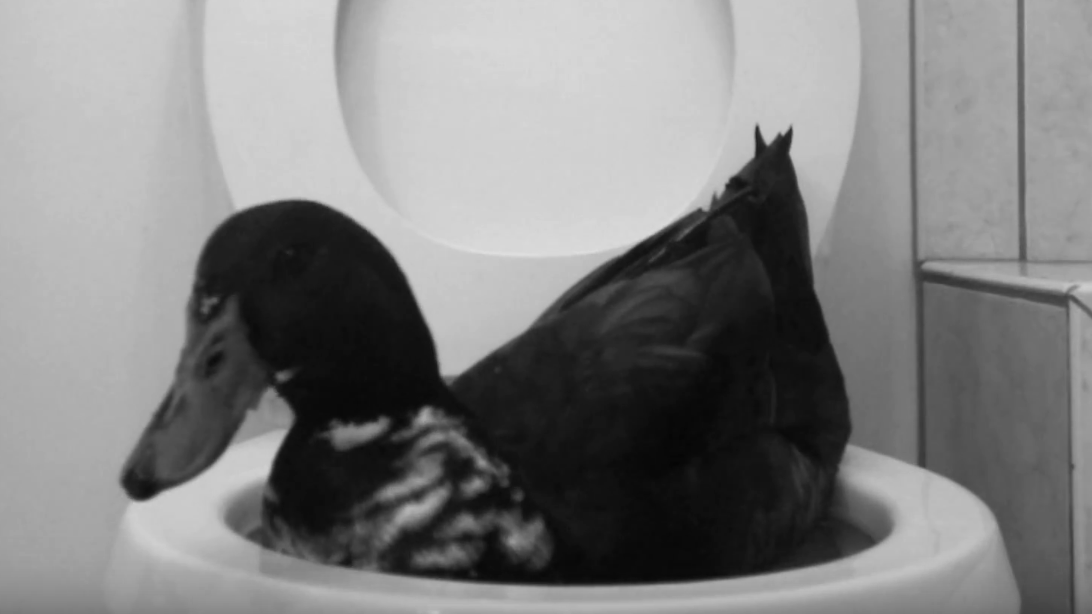
\includegraphics[width=15cm]{bilder/toiletduck.png}			% Titelbild definieren
\end{textblock}

\begin{textblock}{154}(28,133.5)
	\begin{picture}(150,2)
		\put(0,0){\color{bfhgrey}\rule{150mm}{2mm}}
	\end{picture}
\end{textblock}
\color{black}

% Institution / Titel / Untertitel / Autoren / Experten:
%---------------------------------------------------------------------------
\begin{flushleft}

\vspace*{115mm}

\fontsize{26pt}{28pt}\selectfont 
\titel 				\\							% Titel aus der Datei vorspann/titel.tex lesen
\vspace{2mm}

\fontsize{16pt}{20pt}\selectfont\vspace{0.3em}
Smart Toilet 2.0\\							% Untertitel eingeben
\vspace{5mm}

\fontsize{10pt}{12pt}\selectfont
\textbf Business plan\\									% eingeben
\vspace{3mm}

% Abstract (eingeben):
%---------------------------------------------------------------------------
\begin{textblock}{150}(28,190)
\fontsize{10pt}{12pt}\selectfont
Smoilet 2.0 erm�glicht es das Sp�len jeder beliebiger Toilette an das Internet of Things anzuschliessen und er�ffnet eine komplett neue Dimension der Heimautomation. Smoilet 2.0 ist einfach zu bedinen und integriert sich ohne grossen Aufwand.
\end{textblock}

\begin{textblock}{150}(28,225)
\fontsize{10pt}{17pt}\selectfont
\begin{tabbing}
xxxxxxxxxxxxxxx\=xxxxxxxxxxxxxxxxxxxxxxxxxxxxxxxxxxxxxxxxxxxxxxx \kill
Studiengang:	\> BSc Informatik	\\			% Namen eingeben
Autoren:		\> Sebastian Plattner, Patrik Marti, Claudio Deluca, Simon Pf�ffli, Valentina Lanz, Mischa Lehmann 		\\					% Namen eingeben
Betreuer:	\> 	Roland Burri, Daniel Huber	\\					% Namen eingeben
Auftraggeber:	\> BZG4205/06						\\					% Namen eingeben
Experten:		\> Roland Burri, Daniel Huber				\\					% Namen eingeben
Datum:			\> \versiondate					\\		% aus Datei vorspann/version.tex lesen
\end{tabbing}

\end{textblock}
\end{flushleft}

\begin{textblock}{150}(28,280)
\noindent 
\color{bfhgrey}\fontsize{9pt}{10pt}\selectfont
Berner Fachhochschule | Haute �cole sp�cialis�e bernoise | Bern University of Applied Sciences
\color{black}\selectfont
\end{textblock}


\end{titlepage}

%
% ===========================================================================
% EOF
%
			% activate for Titelseite mit Bild
% Versionenkontrolle :
% -----------------------------------------------

\begin{textblock}{180}(15,150)
\color{black}
\begin{huge}
Versionen
\end{huge}
\vspace{10mm}

\fontsize{10pt}{18pt}\selectfont
\begin{tabbing}
xxxxxxxxxxx\=xxxxxxxxxxxxxxx\=xxxxxxxxxxxxxx\=xxxxxxxxxxxxxxxxxxxxxxxxxxxxxxxxxxxxxxxxxxxxxxx \kill
Version	\> Datum	\> Status		\> Bemerkungen		\\
0.1	\> 30.03.2016	\> Entwurf		\> Dokumentinitialisierung	\\	
0.2	\> 13.04.2016	\> Entwurf		\> Arbeit	\\	
\end{tabbing}

\end{textblock}

\cleardoubleemptypage
\setcounter{page}{1}
\cleardoublepage
\phantomsection 
\addcontentsline{toc}{chapter}{Management Summary}
\chapter*{Management Summary}
\label{chap:managementSummary}

Lorem ipsum dolor sit amet, consectetur adipiscing elit. Phasellus scelerisque, leo sed iaculis ornare, mi leo semper urna, ac elementum libero est at risus. Donec eget aliquam urna. Lorem ipsum dolor sit amet, consectetur adipiscing elit. Nunc fermentum nunc sollicitudin leo porttitor volutpat. Duis ac enim lectus, quis malesuada lectus. Aenean vestibulum suscipit justo, in suscipit augue venenatis a. Donec interdum nibh ligula. Aliquam vitae dui a odio cursus interdum quis vitae mi. Phasellus ornare tortor fringilla velit accumsan quis tincidunt magna eleifend. Praesent nisl nibh, cursus in mattis ac, ultrices ac nulla. Nulla ante urna, aliquet eu tempus ut, feugiat id nisl. Nunc sit amet mauris vitae turpis scelerisque mattis et sed metus. Aliquam interdum congue odio, sed semper elit ullamcorper vitae. Morbi orci elit, feugiat vel hendrerit nec, sollicitudin non massa. Quisque lacus metus, vulputate id ullamcorper id, consequat eget orci \nocite{kopka:band1} \nocite{Marti06}. 

\cleardoubleemptypage
%---------------------------------------------------------------------------

% Table of contents
%---------------------------------------------------------------------------
\tableofcontents
\cleardoublepage
%---------------------------------------------------------------------------

% Main part:
%---------------------------------------------------------------------------
\pagenumbering{arabic}
\chapter{Strategie}
\label{chap:strategie}

\begin{center}
	\textit{"Better toilets for a better Future. "}
\end{center}

\section{Unternehmung}
\label{sec:unternehmung}

Unsere Mission ist es mit Smoilet 2.0 die ordin�re Toilette an das Internet of Things anzuschliessen. Die Unternehmung wurde am 1. April 2016 von sechs Studenten, der Fachrichtung Informatik ins Leben gerufen. Gem�ss unseres Leitbildes setzen wir stark auf die Nachhaltigkeit in allen Aspekten.

\begin{figure}[H]
	\centering
	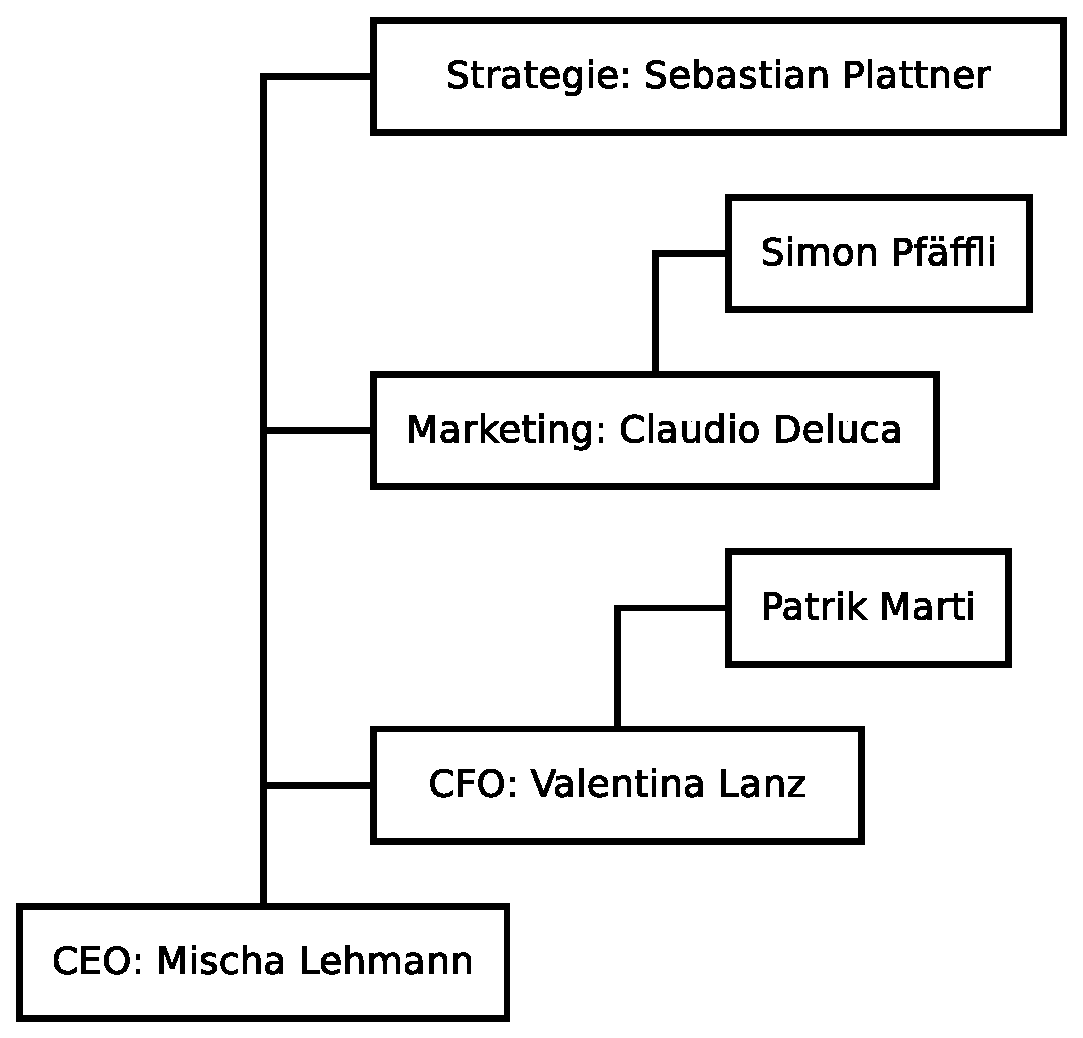
\includegraphics[scale=0.5]{bilder/organisation}
	\caption{Organigramm}
	\label{fig:organigramm}
\end{figure}

\section{Umgebungsanalyse}

SWOT

\section{Marktanalyse}

5 Forces

\section{Selbstanalyse}

Differential SWOT
\chapter{Markt}
\label{chap:markt}

\section{Markpotential}

Weltweit haben ca. 40\% Zugang zu einer Sp�ltoilette, bei einer ungef�hren Bev�lkerung von etwa 7 Milliarden Personen, ergibt das etwa 2.8 Milliarden Personen mit Zugang zu einer Sp�ltoilette. Wenn wir annehmen, dass alle Haushalte mindestens eine Toilette haben, plus alle Toiletten in Gesch�ften, Schulen, �ffentlichen Geb�uden, gibt das min. eine Toilette pro zwei Personen. Somit gibt es weltweit ca 1.4 Milliarden Toiletten.

Als Markt werden L�nder angestrebt mit einem hohen Interesse an Technologie. Zu beginn konzentrieren wir uns auf die deutschsprachigen L�nder:

\begin{itemize}
\item Schweiz (ca. 8 Millionen)
\item Deutschland (ca. 80 Millionen)
\item �sterreich (ca 8.5 Millionen)
\end{itemize}

Das ergibt Total ca. 96 Millionen Einwohner. Wenn wir uns das Alterssegment zwischen 20 und 39 Jahren anschauen (In der Schweiz sind das gem�ss BFS \footnote{\url{http://www.bfs.admin.ch/bfs/portal/de/index/themen/01/02/blank/key/alter/gesamt.html}} ca. 25\% der Bev�lkerung) bleiben ca. 24 Millionen Einwohner �brig.
Wir denken das Smoilet 2.0 haupts�chlich von Techniker oder Personen mit gleichrangigen berufen benutzt wird. Gem�ss BFS \footnote{\url{http://www.bfs.admin.ch/bfs/portal/de/index/themen/01/07/blank/ind43.indicator.43052.430108.html}} sind das ca 20\% und somit ca 5. Millionen Einwohner.

Das ergibt mit den oben genannten Zahlen (min. eine Toilette pro zwei Personen) etwa 2.5 Millionen Toiletten.

\section{Marktanteil}

F�r unsere Crowdfunding Kampagne streben wir den Verkauf von 10'000 Smoilet 2.0 Ger�ten an (0.4\% Marktanteil).
Anschliessend planen wir einen Wachstum von 50\% pro Jahr.

Das ergibt folgende Marktanteile.

1. Jahr 10'000 Einheiten 0.4 Prozent
2. Jahr 15'000 Einheiten 1 Prozent
3. Jahr 22'500 Einheiten 1.9 Prozent

% Todo Make Table!

\section{Bed�rfnisse}

Haushaltsger�te sollen heutzutage nicht mehr nur langweilige Ger�te sein, welche eine einfache Aufgabe erf�llen. K�hlschr�nke sind beispielsweise nicht mehr nur K�hlger�te. Sie denken mit und unterst�tzen den Besitzer bei den n�tigen Eink�ufen oder nehmen ihm sogar solche Aufgaben ab. So soll es auch mit der Toilette sein. Es gibt schon zahlreiche Produkte welche den Comfort der Toilettenbesucher erh�hen. Dies ist allerdings nicht das Ziel des Produktes. Smoilet soll Informationen zur Benutzung der Toilette liefern. Die Bed�rfnisse unserer Abnehmer lassen sich in folgende Kategorien unterteilen:
\begin{itemize}
\item �kologisch: Interesse an den Auswirkungen der Toilette auf die Umwelt.
\item Wirtschaftlich: M�gliches Sparpotenzial.
\item Wartung: Materialverbrauch, Abn�tzung.
\item Just for fun: Basteleien.
\end{itemize}

Diese Bed�rfnisse k�nnen alle komplett oder zum Teil durch unser Produkt abgedeckt werden.

\section{Konkurrenz}
Es gibt bereits zahlreiche Gadgets f�r die eigene Toilette zu kaufen. Die oben Beschriebenen Bed�rfnisse werden aber nicht oder kaum abgedeckt. Einzelne Prototypen wurden zwar schon entwickelt, sind aber nicht f�r den einfachen Toilettenbesitzer zug�nglich (https://twitter.com/shithappen, https://twitter.com/miketoilet, https://twitter.com/hacklabTOilet). 
\chapter{FInanzen}
\label{chap:finanzen}

\section{Finanzierungskonzept}
\section{Steuern}
\section{Zukunft}
\section{Tabellen}
\chapter{Schluss}
\label{chap:schluss}

\section{Strategie}

Im die PEST-Analyse zeigt, dass Smoilet in der Schweiz keinen speziellen Regulierungen unterliegt. Eine grosse Gefahr ist die direkte Konkurrenz durch etablierte Player auf dem Toilettenmarkt. Wir wollen diese Problematik aber entsch�rfen in dem wir von Anfang an auf eine Kooperation mit einem m�glichen Konkurrenten hinarbeiten.

\section{Markt}

Sp�ltoiletten sind weltweit verbreitet und der Absatzmarkt riesig. Jedoch ist die Einstellung zur Toilette stark von Kulturellen Aspekten gepr�gt und unterscheidet sich regional stark. Wir m�ssen bei der Marktbereitung jeweils penibel darauf achten den entsprechenden Markt richtig zu bearbeiten. Das Produkt soll in zwei Varianten erh�ltlich sein wobei f�r jede Variante ein unterschiedlicher Absatzkanal vorgesehen ist. Das Produkt soll erst einen Techie-Lifestyle vermitteln, mit steigender Maturit�t aber zum zuverl�ssigen Produkt weiterentwickelt werden.

\section{Finanzen}

Ziel des Crowdfundings liegt nicht prim�r in der Umsatzsteigerung, sondern in der Gewinnmaximierung durch Kostenersparnisse in Bezug auf Werbung und Kundensuche. In unserer Kostenrechnung stellten wir fest, dass die reine Finanzierung durch Crowdfunding nicht realistisch ist. Zur L�sung dieses Problems haben wir zwei Varianten erarbeitet. Von welchen wir die Variante ,,Startfinanzierung durch Investoren`` bevorzugen.

\section{Weiteres Vorgehen}

Unsere Strategie sieht einen streng Timeboxed Ansatz vor. Wichtig dabei sind die strikten Meilensteinen. Sollte ein Meilenstein nicht erreicht werden, brechen wir das Projekt ab.

\begin{figure}[H]
	\centering
	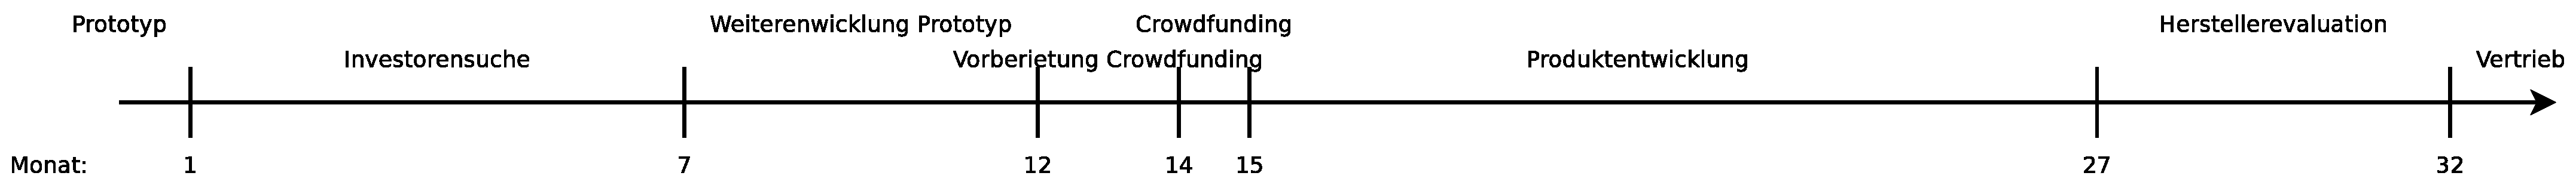
\includegraphics[width=\textwidth]{bilder/timeline}
	\caption{Timeline}
	\label{fig:timeline}
\end{figure}

\paragraph{Prototyp} Entwicklung eines Protoypen der die grunds�tzliche Machbarkeit aufzeigt. Ziel der Phase ist es einen Tweet beim Sp�len einer herk�mmlichen Toilette auszul�sen.

\paragraph{Investorensuche} Wir suchen mindestens einen Geldgeber der uns gen�gend unterst�tzt damit wir uns L�hne bis zur Vertriebsphase auszahlen k�nnen. Weiter soll in dieser Phase mindestens ein Partner f�r die OEM-Variante evaluiert werden.

\paragraph{Weiterentwicklung Prototyp} Wir entwickeln den Prototyp soweit weiter, dass dieser in der Crowdfunding-Phase Erfolg haben kann. Wir legen speziell Wert darauf die einfache Integration zu f�rdern und eine ansprechendes Design zu entwickeln. Ziel dieser Phase ist es einen ersten Anwender zu finden welchen wir vom Produkt �berzeugen k�nnen, so dass dieser das Produkt selbst nach dieser Phase installiert l�sst.

\paragraph{Vorbereitung Crowdfunding} Wir setzen eine Internetpr�senz und einen Social-Media auftritt auf. Ziel dieser Phase ist es, dass ein m�glicher Interessent auf eine Website mit Video verlinkt werden kann.

\paragraph{Crowdfunding} Ziel ist es das Funding-Goal zu erreichen.

\paragraph{Produktentwicklung} Smoilet 2.0 wird zum vertriebsf�higen Produkt: Neben den im Crowdfunding versprochenen Features muss eine Dokumentation, diverse Anwendungsf�lle und die E-Commerce Plattform aufgebaut werden.

\paragraph{Herstellerevaluation} Wir evaluieren einen Hersteller der Smoilet 2.0 produziert.

\paragraph{Vertieb} Mit dem Geld der Crowdfunding-Kampagne wird eine erster Batch Smoilet 2.0 produziert. Dieser Batch beinhaltet ein Smoilet 2.0 f�r jeden G�nner sowie einige Ger�te die �ber OEM-Kan�le vertrieben werden. Mit dem Absatz des OEM-Verkaufes finanzieren wir den n�chsten Badge an Smoilet 2.0.






%---------------------------------------------------------------------------

% Glossary
%---------------------------------------------------------------------------
\cleardoublepage
\phantomsection 
\addcontentsline{toc}{chapter}{Glossar}
\renewcommand{\glossaryname}{Glossar}
\printglossary
%---------------------------------------------------------------------------

% Bibliography
%---------------------------------------------------------------------------
\cleardoublepage
\phantomsection 
\addcontentsline{toc}{chapter}{Literaturverzeichnis}
\bibliographystyle{IEEEtranS}
\bibliography{datenbanken/bibliography}{}
%---------------------------------------------------------------------------

% Listings
%---------------------------------------------------------------------------
\cleardoublepage
\phantomsection 
\addcontentsline{toc}{chapter}{Abbildungsverzeichnis}
\listoffigures
\cleardoublepage
\phantomsection 
\addcontentsline{toc}{chapter}{Tabellenverzeichnis}
\listoftables
%---------------------------------------------------------------------------

% Index
%---------------------------------------------------------------------------
%\cleardoublepage
%\phantomsection 
%\addcontentsline{toc}{chapter}{Stichwortverzeichnis}
%\renewcommand{\indexname}{Stichwortverzeichnis}
%\printindex
%---------------------------------------------------------------------------

% Attachment:
%---------------------------------------------------------------------------
\appendix
\settocdepth{section}
%---------------------------------------------------------------------------

%---------------------------------------------------------------------------
\end{document}

